\documentclass[a4paper,12pt,bold]{scrartcl}

\renewcommand{\baselinestretch}{1.3}\normalsize
\newcommand{\vect}[1]{\mathbf{#1}}
\newcommand{\thin}{\thinspace}
\newcommand{\thick}{\thickspace}
\newcommand{\N}{\mathcal{N}}	%Normal Distribution
\newcommand{\U}{\mathrm{U}}	%Uniform Distribution
\newcommand{\D}{\mathrm{D}}	%Dirichlet Distribution
\newcommand{\W}{\mathrm{W}}	%Wishart Distribution
\newcommand{\E}{\mathrm{E}}		%Expectation
\newcommand{\Iden}{\mathbb{I}}	%Identity Matrix
\newcommand{\Ind}{\mathrm{I}}	%Indicator Function

\newcommand{\bs}{\boldsymbol}
\newcommand{\var}{\mathrm{var}\thin}
\newcommand{\plim}{\mathrm{plim}\thin}
\newcommand{\cov}{\mathrm{cov}\thin}
\newcommand\indep{\protect\mathpalette{\protect\independenT}{\perp}}
\def\independenT#1#2{\mathrel{\rlap{$#1#2$}\mkern5mu{#1#2}}}
\usepackage{bbm}
%\usepackage{endfloat}
\renewcommand{\vec}[1]{\mathbf{#1}}



\parindent0pt
\usepackage{algpseudocode,tabularx,ragged2e}
\newcolumntype{C}{>{\centering\arraybackslash}X} % centered "X" column
\newcolumntype{L}{>{\arraybackslash}X} % centered "X" column

\usepackage{algorithmicx}
\usepackage{graphicx}
\usepackage{afterpage}

\usepackage{algorithm}
\graphicspath{{../code/}}

\usepackage{float}
\usepackage[section]{placeins}
\usepackage{apacite}
\usepackage{booktabs}
\usepackage{epigraph}
\usepackage[sans]{dsfont}
\usepackage[round,longnamesfirst]{natbib}
\usepackage{bm}																									%matrix symbol
\usepackage{setspace}																						%Fu�noten (allgm.
\usepackage[colorlinks = true,
            linkcolor = blue,
            urlcolor  = blue,
            citecolor = blue,
            anchorcolor = blue]{hyperref}%Zeilenabst�nde)
\usepackage{threeparttable}
\usepackage{lscape}																							%Querformat
\usepackage[latin1]{inputenc}
													%Umlaute
\usepackage{graphicx}
\usepackage{amsmath}
\usepackage{amssymb}
\usepackage{fancybox}																						%Boxen und Rahmen
\usepackage{appendix}
\usepackage{listings}
\usepackage{xr}
\usepackage{pdflscape}

\usepackage{enumerate}
\usepackage[labelfont=bf]{caption}
																		%EURO Symbol
\usepackage{tabularx}
\usepackage{longtable}
\usepackage{subfig,float}																				%Mehrseitige Tabellen
\usepackage{color,colortbl}																			%Farbige Tabellen
\usepackage[left=3cm, right=2cm, top=2cm, bottom=2.5cm]{geometry} %Seitenr�nder
%\usepackage[normal]{caption2}[2002/08/03]												%Titel ohne float - Umgebung
\definecolor{lightgrey}{gray}{0.95}	%Farben mischen
\definecolor{grey}{gray}{0.85}
\definecolor{darkgrey}{gray}{0.80}

\newcommand{\mc}{\multicolumn}
\usepackage{rotating}

\usepackage{tikz}
\usetikzlibrary{positioning}
\usepackage[export]{adjustbox}

\usepackage{caption}
\captionsetup[figure]{labelfont=bf}

\usepackage{url}  % Used for linebreaks in verbatim statements
\usepackage{multirow}

\newtheorem{Definition}{Definition}
\newtheorem{Remark}{Remark}
\newtheorem{Lemma}{Lemma}
\newtheorem{Theorem}{Theorem}
\newtheorem{Assumption}{Assumption}
\newtheorem{Excercise}{Excercise}
\newtheorem{Result}{Result}
\newtheorem{Proposition}{Proposition}
\newtheorem{Prediction}{Prediction}
\newtheorem{Solution}{Solution}
\newtheorem{Problem}{Problem}

\setlength{\skip\footins}{1.0cm}
\deffootnote[1em]{1.1em}{0em}{\textsuperscript{\thefootnotemark}}
\renewcommand{\arraystretch}{1.05}

\DeclareMathOperator*{\argmin}{arg\,min}
\DeclareMathOperator*{\argmax}{arg\,max}




\newenvironment{boenumerate}
{\begin{enumerate}\renewcommand\labelenumi{\textbf{(\theenumi)}}}
{\end{enumerate}}
\makeatletter
\newenvironment{manquotation}[2][2em]
  {\setlength{\@tempdima}{#1}%
   \def\chapquote@author{#2}%
   \parshape 1 \@tempdima \dimexpr\textwidth-2\@tempdima\relax%
   \itshape}
  {\par\normalfont\hfill--\ \chapquote@author\hspace*{\@tempdima}\par\bigskip}



\setkomafont{author}{\scshape}
\usepackage{blindtext}

\title{Project description of my thesis on a robust approach to John Rust's 1987 optimal replacement of bus engines}
\author{Maximilian Blesch}
\date{\today}



\begin{document}
\maketitle
\newpage
\tableofcontents
\newpage
\section{Introduction}
This paper summarizes the progress of my thesis and will provide a short outlook on the aim of the project. The thesis takes a second look at \cite{Rust.1987} to explore if alternative decision rules can outperform the decision rule deviated from Bellman's equation. As Rust was the first to implement a Nested Fixed Point Algorithm and therefore solved Bellman's decision problem computationally, his paper is an adequate representative to show the power of a robust implementation in this class of models. The mathematical tools for the alternative decision rules are mainly inspired by Chapter 13 of \cite{Ben-Tal.2009}, but also by applications from other fields such as \cite{Kaufman.2017} or \cite{Ben-Tal.2011}. This handout will be continuously updated as more steps are completed and presented at different occasions. It was first used during a Hackathon in the Open Source Economics research group at the Institute for Applied Microeconomics and this current version is presented as a seminar paper for the Effective Programming Practice course of Professor Hans-Martin von Gaudecker. In the first chapter of this paper I will shortly introduce the data John Rust used and then give a short summary of the assumptions and results that form the model in \cite{Rust.1987}. In the third chapter I will provide some replication results to show the quality of my Nested Fixed Point Algorithm. For the fourth chapter, I implemented a simulation option to my package and introduced a performance measure of a decision rule. This is the current state of the project and in the last chapter I will present a rough outlook on the upcoming steps.

\section{Original data by John Rust}
The first part of my thesis was the pyhton implementation of the Nested Fixed Point Algorithm (NFXP). To test my algorithm, I replicated the paper of John Rust. The data in the paper is provided by the agent, whose decision rule Rust estimated, the maintenance manager of the Madison (Wisconsin,US) Metropolitan Bus Company, Harold Zurcher. He provides Rust with a sample of 162 buses from December 1974 to May 1985. The data consists of monthly observations on the odometer readings for each bus, plus data on the date and odometer readings at which a bus engine was replaced. John Rust kindly provides access to this data on his homepage. Rust divides his sample of buses by make, model and year of purchase into 8 groups. To find out which group corresponds to which model please refer to Table 1 of \cite{Rust.1987}. As these details are not important for the further analysis, I will just refer to the groups. To verify my data reading process I replicated some descriptives Tables of \cite{Rust.1987}:

\newpage

\begin{table}[h]
\begin{center}
  \input{figures/descr_2a.txt}
  \caption{Table 2a of \cite{Rust.1987}: \\ Buses with at least 1 engine replacement}
\end{center}
\end{table}
The table above deviates from the original table in the maximal and minimal value in the full sample row. As these numbers should agree with the maximal and minimal number from the rows above, it is safe to say that this is due to a typo by John Rust. \\
\begin{table}[h]
\begin{center}
  \input{figures/descr_2b.txt}
  \caption{Table 2b of \cite{Rust.1987}: \\ Buses with no replacement}
\end{center}
\end{table}

\newpage
\section{Model of optimal replacement}
Rust chooses the following theoretical framework: Notation wise he refrains from using superscripts indicating the buses, as he assumes that there is complete independence of the decisions made for each bus. In every month (from now on called period) the agent, Harold Zurcher, has the choice to either replace (\(i_t = 1 \)) or to maintain (\(i_t = 0\)) a bus. The agent chooses an action maximizing his objective function, i.e. the current value of the bus (Bellman equation):
\begin{equation} \label{eq:1}
  V_{\theta}(x_t, \varepsilon_t) = \sup_{\prod} E [\sum_{j=t}^{\infty} \beta^{j-t} (u(x_j, i_j, \theta_1) + \varepsilon_j(i_j))| x_t, \varepsilon_t, \theta_2, \theta_3]
\end{equation}
with
\begin{equation}
  u(x_t,i_t, \theta)=
  \begin{cases}
  -c(x_t, \theta_1)\qquad \qquad  \textbf{if} \quad i_t=0 \\
  -[RC + c(0, \theta_1)]\quad \textbf{if} \quad i_t=1
  \end{cases}
\end{equation}
where $\prod = \{i_t, i_{t+1}, ...\}$. John Rust shows in \cite{Rust.1988}, that under certain regularity assumptions, $i_t$ only depends on $(x_t, \varepsilon_t)$ and does not depend on future decisions. Therefore \ref{eq:1} can be rewritten:
  \begin{equation} \label{eq:2}
    V_{\theta}(x_t, \varepsilon_t) = \max_{i_t \in \{0, 1\}} [ u(x_t, i_t, \theta) + \varepsilon_t (i_t) + \beta EV_{ \theta }( x_t, \varepsilon_t, i_t) ]
  \end{equation}
with
\begin{equation}
  EV_{\theta}(x_t, \varepsilon_t, i_t) = \int_{\gamma}\int_{\eta} V_{\theta}(\gamma, \eta)p(d\gamma, d\eta | x_t, \varepsilon_t, i_t, \theta_2, \theta_3),
\end{equation}
  \bigskip
where \\
\begin{table}[htbp]
    \centering % to have the caption near the table
    \begin{tabular}{l c p{10cm} }
        $x_t$ & : & Mileage on the odometer of the bus in period $t$\\
        $\varepsilon_t$ & : & Unobserved utility for each decision in period $t$\\
        $\mathbf{EV}_{\theta}$ & : & Future expected value of each decision\\
    \end{tabular}
\end{table}

and $\theta = \left(\theta_1, \theta_2, \theta_3, \mathbf{RC}, \beta \right)$ is the vector of the unknown variables to be estimated.



\begin{table}[htbp]
    \centering % to have the caption near the table
    \begin{tabular}{l c p{10cm} }
        $\theta_1$ & : & Cost parameter\\
        $\theta_2$ \& $\theta_3$ & : & Factors that determine the transition probabilities\\
        $\mathbf{RC}$ & : & Replacement costs of a bus engine\\
        $\beta$ & : & Discount factor\\
    \end{tabular}
\end{table}

Further, he assumes conditional independence of the transition probabilities of the error term and the development of mileage (A6 of \cite{Rust.1988}):

\begin{Assumption}
Conditional Independence Assumption(CI):\\
The transition density of the controlled process \(\{x_t, \varepsilon_t\}\) factors as
\begin{equation}
  p(x_{t+1}, \varepsilon_{t+1} | x_t, \varepsilon_t, i_t, \theta_2) = q(\varepsilon_{t+1} | x_{t+1}, \theta_2) p(x_{t+1} | x_t, i_t, \theta_3)
\end{equation}
\end{Assumption}
This theorem involves two restrictions. First, \(x_{t+1}\) is a sufficient statistic for \(\varepsilon_{t+1}\), which implies that any statistical dependence between \(\varepsilon_t\) and \(\varepsilon_{t+1}\) is transmitted entirely through the vector \(x_{t+1}\). Second, the probability density of \(x_{t+1}\) depends only on \(x_t\) and not on \(\varepsilon_t\).\\ The payoff of (CI) is twofold. First, (CI) implies that \(EV_{\theta}\) is not a function of \(\varepsilon_t\), so that the required choice probabilities will not require integration over the unknown function \(EV_{\theta}\). Second, together with the discreization of the state space, (CI) implies that \(EV_{\theta}\) is a fixed point of a separate contraction mapping on the reduced state space \(\{(x, i)| x \in \mathbb{R}^{K} , i \in C(x)\} \), where K is the size of the state space and $C(x)=\{0, 1\}$ is the choice set.\medskip \\
Therefore $x_t$ is the state of the bus in each period t. Furthermore, as the monthly mileage increase in the data is never larger than 15,000, the transition probabilities reduce in the case of a 5000 miles statesize discreization to a multinominal distribution on \{0, 1, 2\}. Rust claims an extreme value distribution  with mean $(0,0)$ and variance $(\pi^2/6, \pi^2/6)$ for $\varepsilon_t$, i.e.
\begin{equation}
  q(\varepsilon_t|x_t, \theta_2) = \prod_{i \in \{0,1\}} exp\{-\varepsilon_t(i) + \theta_2\}exp\{-exp\{-\varepsilon_t(i)+\theta_2\}\}
\end{equation}
$\theta_2 = \gamma = 0.577216$.\\
With the assumptions above and the notation \(EV_{ \theta }( x_t, 1) = EV_{ \theta }( 0, 0) =: EV(0)\) and \(EV_{ \theta }( x_t, 0) =: EV(x_t)\) for all \(x_t\), Rust deviates:
\begin{equation}
  EV_{\theta}(x_t) = \sum_{j \in \{0 ,1, 2\}} p_j * \ln\{ \sum_{i_t \in \{0, 1\}} \exp[u(x_t, i_t, \theta_1, RC) + \beta EV_{\theta}(i_t * (x_t + j))]\}
\end{equation}
with \(p_j\) the transition probabilities to \(j \in \{0,1,2\}\) and for the choice probabilities:
\begin{equation}
P(i_t | x_t, \theta) = \frac{\exp[u(x_t, i_t, \theta_1, RC) + \beta EV_{\theta} (i_t * x_t)]}{ \sum_{i_t \in \{0, 1\}}\exp[u(x_t, i_t, \theta_1, RC) + \beta EV_{\theta} (i_t * x_t)]}
\end{equation}
Furthermore, in \cite{Rust.1988} the author shows that under (CI) the likelihood function for the estimation of \(\theta\) can be split up into two separate functions:
\begin{equation}
  l^1(x_1, .....,  x_T, i_1, ...., i_T | x_0, i_0, \theta) = \prod_{t = 1}^T p(x_t | x_{t-1}, i_{t-1}, \theta_3)
\end{equation}
for the transition probabilities and
\begin{equation}
  l^2(x_1, .....,  x_T, i_1, ...., i_T | \theta) = \prod_{t = 1}^T P(i_t | x_t, \theta_1, RC, \theta_3, \beta)
\end{equation}
for the cost parameters $RC$ and \(\theta_1\). For a detailed proof of the above please, refer to \cite{Rust.1987} and \cite{Rust.1988}.

\section{Replication of \cite{Rust.1987}}
The second step in my thesis is to replicate the paper by Rust and therefore to test my Nested Fixed Point Algorithm. Rust applies his NFXP to three different samples. First he pools groups 1, 2 and 3, then he applies it just to group 4 and in the last step to the pooled group consisting of 1, 2, 3 and 4. In each of these groups the year of purchase is different, thus the number of observed periods in the pooled groups is different for each bus. For the performance evaluation of different decision strategies such a feature is unnecessary, therefore I didn't yet implement this possibility. In the following table I replicated the results for bus group 4 only:
\begin{table}[h]
\begin{center}
  \input{figures/replication.txt}
\end{center}
\end{table}

In the above tables $\beta$ is set fixed and not estimated. Rust argues that the parameter $RC$ and the discount factor $\beta$ both enforce an earlier replacement and therefore are highly co-linear. Thus, treating $\beta$ as a free parameter would result in difficulties for the maximization algorithm. He starts a short discussion, arguing that Zurcher wants to minimize long-run average costs and therefore $\beta$ as a free parameter gets driven to one. It will be an interesting aspect, of how beta influences the performance of different decision strategies.

\section{Performance measure}
The discussion above on the influence of beta on the performance measure, leads me now to the introduction of such a measure. The intuitive step is to evaluate a decision strategy by the expected discounted utility in period $0$. This is of course the value function in time period 0. Rust showed that this value can be calculated with equation \ref{eq:1} and \ref{eq:2}. In the following figure, where I simulated $100$ buses over $100,000$ periods with discount factor $0.9999$, it is shown that these two mathematical expressions agree.
\begin{figure}[h]
\centering
\caption{Convergence of the simulated and calculated $V(0)$}

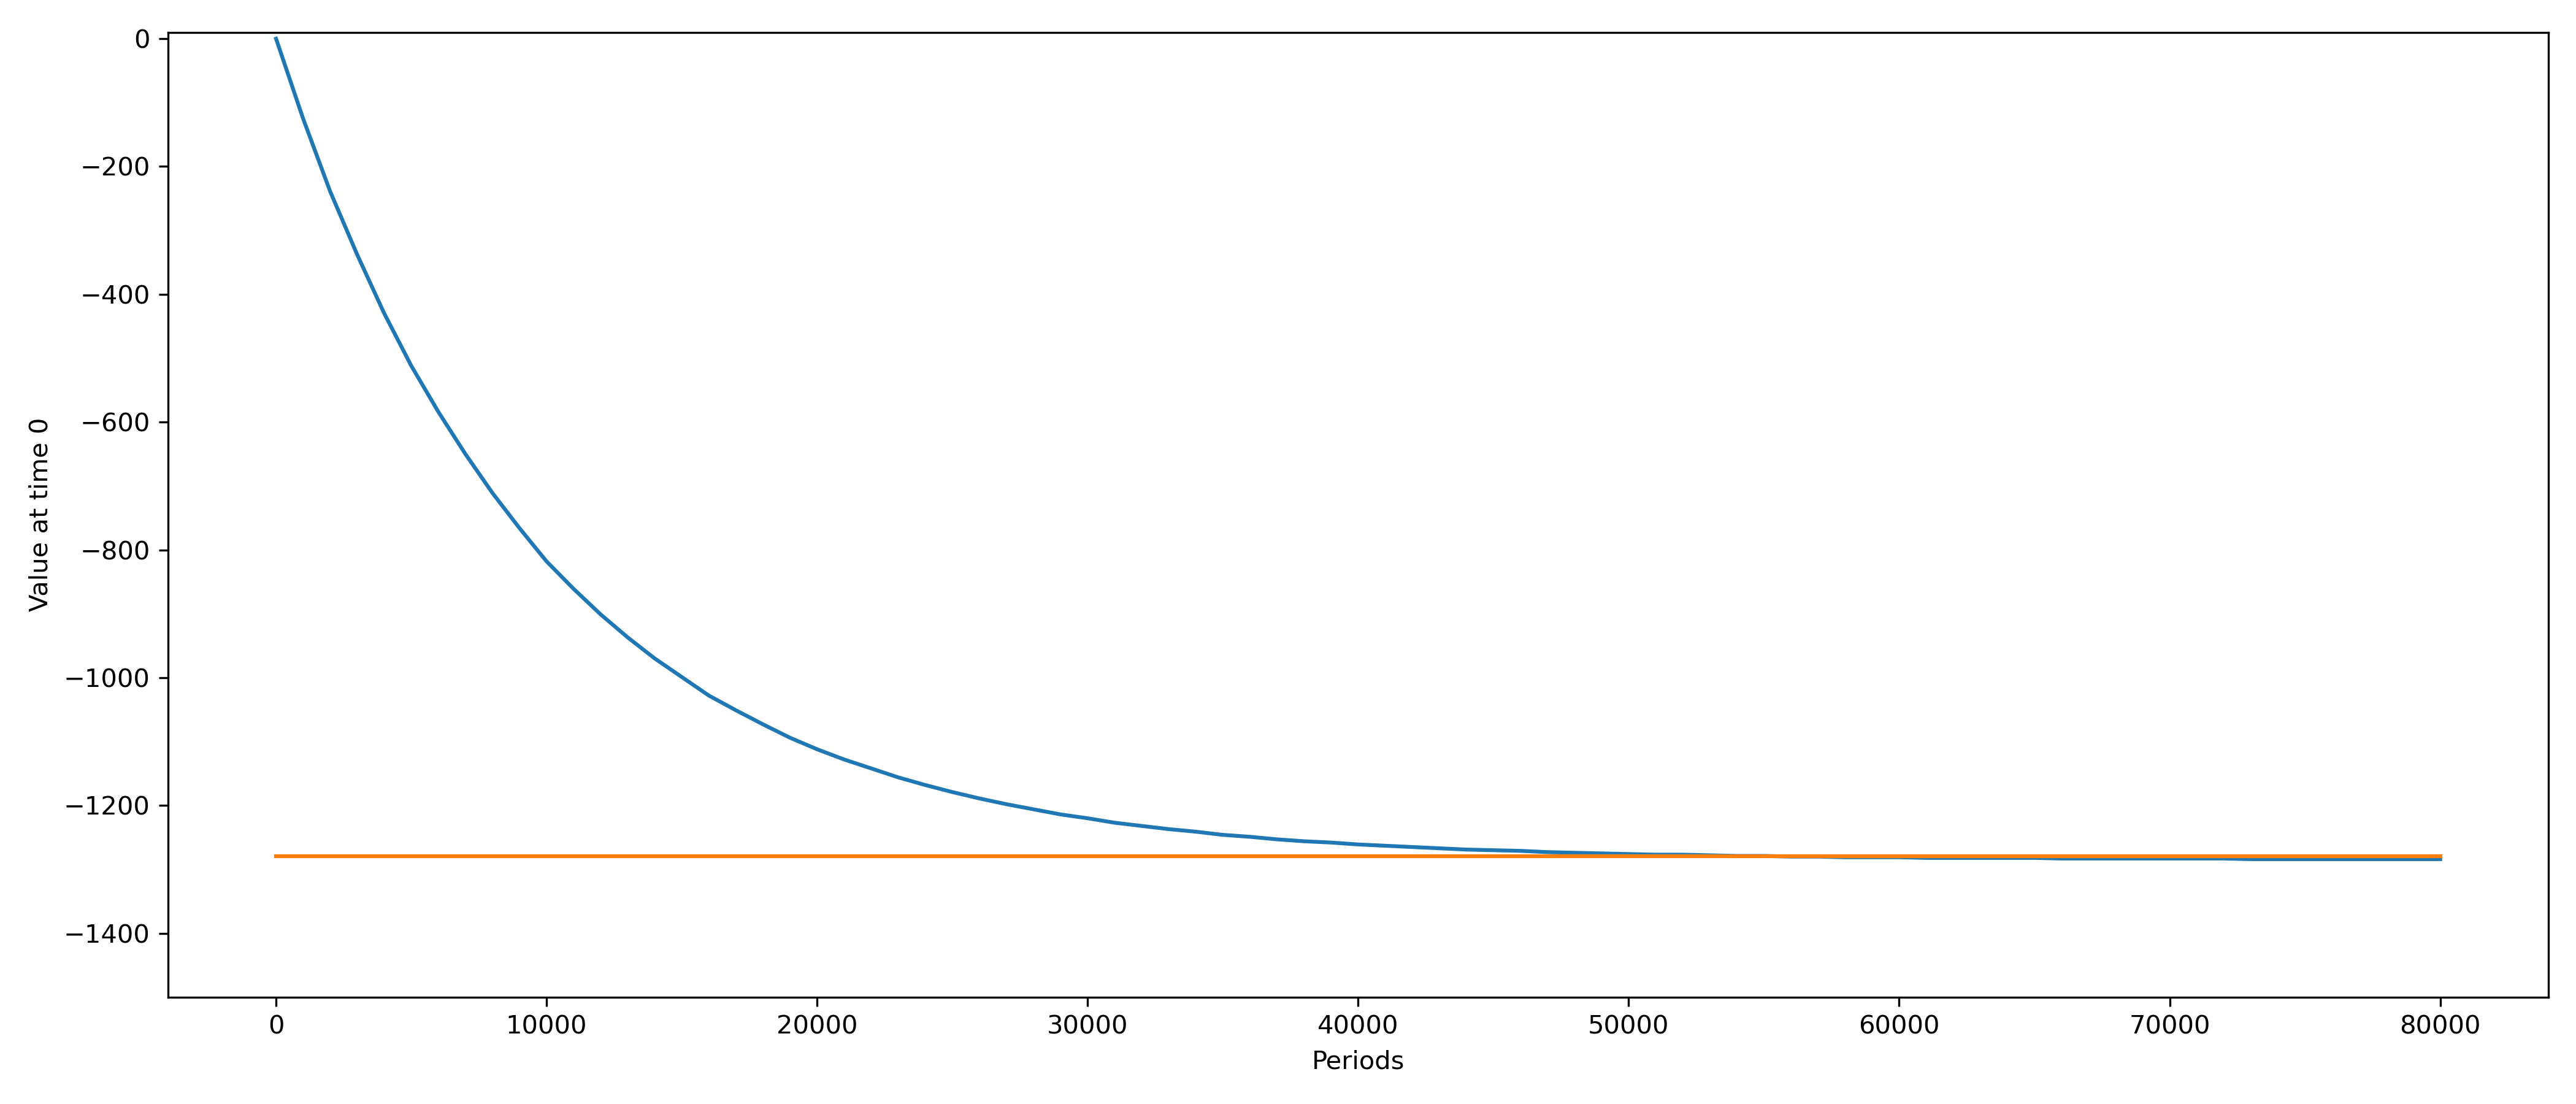
\includegraphics[width=1\linewidth]{figures/figure_1}
\caption{Convergence of the simulated and calculated $V(0)$}
 
\end{figure}

\section{Outlook}
The figure above shows, that if the estimated transition probabilities agree with the real underlying transition probabilities, the expected value calculated by NFXP also agrees with the discounted utility. The next step of my thesis is now to simulate a misbelief of the agent on the transition probabilities. These determine the fixed point $EV(x)$, which the agent uses to choose his optimal action. It will be the scope of my thesis in economics to explore how sensitive the discounted utility and therefore the performance of the decision strategy is, in regards to the deviation of the agent's belief from the true underlying transition probabilities. The aim of the project beyond my thesis will be to develop tools for the agent to anticipate a false belief and therefore outperform the classic decision rule.

\newpage
\bibliographystyle{apacite}
\bibliography{bibliography/literature.bib}

\end{document}
